\ifdefined\isphone
  \documentclass[a6paper,11pt,oneside]{book}

\usepackage{algpseudocode}
\usepackage{algorithm}
\usepackage{amsfonts}
\usepackage{amsmath,amsthm,amssymb}
\usepackage{graphicx}
\usepackage{hyperref}
\usepackage{mathtools}
\usepackage{steinmetz}
\usepackage{fancyvrb}
\usepackage{textcomp}
\usepackage{gensymb}
\usepackage[normalem]{ulem}
\usepackage[T1]{fontenc}
\usepackage{cmap}
\usepackage{xspace}

\DeclareGraphicsExtensions{.pdf,.png,.jpg}

\newcommand{\mb}[1]{\ensuremath{\mathbb{{#1}}}}
\newcommand{\setof}[1]{\ensuremath{\left \{ #1 \right \}}}
\newcommand{\tuple}[1]{\ensuremath{\left \langle #1 \right \rangle }}

\DeclarePairedDelimiter{\ceil}{\lceil}{\rceil}
\DeclarePairedDelimiter{\floor}{\lfloor}{\rfloor}

\DeclareSymbolFont{bbold}{U}{bbold}{m}{n}
\DeclareSymbolFontAlphabet{\mathbbold}{bbold}

\newtheorem{statement}{Statement}
\newtheorem{rmk}{Remark}
\newtheorem{defi}{Definition}
\newtheorem{example}{Example}
\newtheorem{theorem}{Theorem}
\newtheorem{lemma}[theorem]{Lemma}
\newtheorem{proposition}[theorem]{Proposition}
\newtheorem{pf}[theorem]{Proof}
\newtheorem{corollary}[theorem]{Corollary}

% Differences
\usepackage[margin=5mm]{geometry}
\usepackage{tgheros}
\renewcommand*\familydefault{\sfdefault}

\else
  \documentclass[11pt,oneside]{book}

\usepackage{algpseudocode}
\usepackage{algorithm}
\usepackage{amsfonts}
\usepackage{amsmath,amsthm,amssymb}
\usepackage{graphicx}
\usepackage{hyperref}
\usepackage{mathtools}
\usepackage{steinmetz}
\usepackage{fancyvrb}
\usepackage{textcomp}
\usepackage{gensymb}
\usepackage[normalem]{ulem}
\usepackage[T1]{fontenc}
\usepackage{cmap}
\usepackage{xspace}

\DeclareGraphicsExtensions{.pdf,.png,.jpg}

\newcommand{\mb}[1]{\ensuremath{\mathbb{{#1}}}}
\newcommand{\setof}[1]{\ensuremath{\left \{ #1 \right \}}}
\newcommand{\tuple}[1]{\ensuremath{\left \langle #1 \right \rangle }}

\DeclarePairedDelimiter{\ceil}{\lceil}{\rceil}
\DeclarePairedDelimiter{\floor}{\lfloor}{\rfloor}

\DeclareSymbolFont{bbold}{U}{bbold}{m}{n}
\DeclareSymbolFontAlphabet{\mathbbold}{bbold}

\newtheorem{statement}{Statement}
\newtheorem{rmk}{Remark}
\newtheorem{defi}{Definition}
\newtheorem{example}{Example}
\newtheorem{theorem}{Theorem}
\newtheorem{lemma}[theorem]{Lemma}
\newtheorem{proposition}[theorem]{Proposition}
\newtheorem{pf}[theorem]{Proof}
\newtheorem{corollary}[theorem]{Corollary}

% Differences
\setlength{\textheight}{9.5in}
\setlength{\textwidth}{7.0in}
\setlength{\topmargin}{-0.75in}
\setlength{\oddsidemargin}{-0.25in}
\setlength{\evensidemargin}{0.75in}
\setlength{\parskip}{0.15in}
\setlength{\parindent}{0in}

\fi

\usepackage{listings}
\usepackage{imakeidx}

\makeindex

% Course Name
\title{STAT 206}

% Fill in your name.
\author{Shale Craig}

% Set the default pseudocode language:
\lstset{language=Python}

\newcommand{\ex}{\textbf{Example:} }

% Now we will begin writing the document.
\begin{document}
    \maketitle

    % Next, we need to make a Table of Contents, List of Figures and
    % List of Tables.  You will most likely need to run LaTeX twice to
    % get these correct.  The first pass for LaTeX to figure out the
    % labels, and the second pass to put in the right references.
    \tableofcontents

    %%%%%%%%%%%%%%%%%%%%%%%%%%%%%%%%%%%%%%%%%%%%%%%%%%%%%%%%%%%%%%%%%%%%%
    %% REPORT BODY
    %%%%%%%%%%%%%%%%%%%%%%%%%%%%%%%%%%%%%%%%%%%%%%%%%%%%%%%%%%%%%%%%%%%%%
    %% \main will make the \section commands numbered again,
    %% it will also use arabic page numbers.
    \mainmatter

    \part{Content Before Midterm 1} % (fold)
    \label{prt:content_ _before_ _midterm_ _1_}
        \chapter{Getting Acquainted with Statistics} % (fold)
        \label{cha:getting_acquainted_with_statistics}
            \section{Definitions} % (fold)
            \label{sec:definitions}
                Empirical Studies are algorithms of the form: \emph{Hypothesi} $\to$ \emph{Data Collection} $\to$ \emph{Analysis}.
                For example, we may ask:
                \begin{quote}
                    Can people tell if vinyl sounds better than MP3?
                \end{quote}
                \begin{description}
                    \item[Unit]\index{unit} is a single element (i.e. model, entity, person, item, etc) of a population whose characteristics we are interested in.
                    \item[Population]\index{population} is the universe of all \emph{Unit}s we are interested in.
                    \item[Variables]\index{variables} are a measurement of the characteristic from a unit.
                \end{description}
                After some class discussion, we change the question to be as follows:
                \begin{quote}
                    Can healthy teens tell if vinyl sounds better than mp3?
                \end{quote}
                In this question, here are the different sections:
                \begin{description}
                    \item[Population] All healthy teens
                    \item[Unit] A single healthy teen
                    \item[Variable 1] Can the Unit correctly identify the recognized type?
                    \item[Variable 2] Which recording did the Unit believe sounds better?
                \end{description}
                We define the following other terms:
                \begin{description}
                    \item[Categorial Variable:]\index{categorial variable} qualitative variable, belongs to $k$ classes or categories.
                    \item[Discrete Variable:]\index{discrete variable} quantitative, countable variable (Integers).
                    \item[Continuous Variable:]\index{continuous variable} quantitative, non-countable (Reals).
                    \item[Sample:]\index{sample} A subset of the population from which measurements are actually made.
                    \item[Sample Error:]\index{sample error} The error introduced by estimating an entire population's characteristics from a \emph{Sample}.
                    \item[Study Error:]\index{study error} A systematic, \emph{unfixable} error through the sample not accurately representing the population.
                \end{description}

                There are these metrics:
                \begin{description}
                    \item[Sample Mean:]\index{mean} $\bar{x} = \sum_{i \in 1}^{n} x_i$.
                    \item[Median:]\index{median}\index{x@$\bar{x^*}$} (middle point)
                        \begin{align*}
                        x^* &= \left\{
                             \begin{array}{lr}
                               x_{\frac{n+1}{2}} & : \text{if $n$ is odd} \\
                               \frac{x_{\frac{n+1}{2}} + x_{\frac{n+2}{2}}}{2} & : \text{if $n$ is even}
                             \end{array}
                           \right.
                    \end{align*}
                    \item[Sample Variance:]\index{variance}\index{dispersion}\index{s!s2@$s^2$} $s^2 = \frac{\sum_{i=1}^n (x_i - \bar{x})^2}{n-1}$
                    \item[Standard Deviation:]\index{standard deviation}\index{s@$s$} $s = \sqrt{s^2}$
                    \item[Range:] $x_n - x_1$ (max - min)
                \end{description}

                There are two different kinds of Statistics:
                \begin{description}
                    \item[Descriptive Statistics]\index{descriptive statistics} is summarizing data from a sample both graphically and numerically.
                    \item[Inferential Statistics]\index{inferential statistics} uses a sample to generalize results to the entire population.
                \end{description}
            % section definitions (end)

            \section{Probability} % (fold)
            \label{sec:probability}
                Classic probability is usually defined as:
                \begin{align*}
                    \frac{\text{Number of ways event can occur}}{\text{Total number of equally likely outcomes}}
                \end{align*}

                \begin{description}
                    \item[Relative Frequency:]\index{relative frequency} the proportion of times outcome occurs as a number of trials approaches infinity.
                    \item[Subjective Frequency:]\index{subjective frequency} estimates of probability based on subjective opinion.
                    \item[Experiment:]\index{experiment} is a repeatable phenomenon
                    \item[Trial:]\index{trial} is a single instance of an experiment
                    \item[Sample Space:]\index{sample space} is the set of distinct outcomes for an experiment or process where only one outcome of the set occurs
                        \begin{description}
                            \item[Discrete] sample spaces have countable number of simple event
                            \item[Non-Discrete/Continuous] sample spaces have a non-countable number of simple events
                        \end{description}
                \end{description}

                Experiment: Flip a coin 3 times.
                \subsection{Probability Models} % (fold)
                \label{sub:probability_models}
                    \begin{align*}
                        (\forall A) & (0 \le P(A) \le 1)
                    \end{align*}
                    If $A$ and $B$ are \emph{mutually exclusive} events, then:
                    \begin{align*}
                        P(A \cup B) &= P(A) + P(B)
                    \end{align*}

                    The distribution for finite sample space $S = \{ a_1, a_2, a_3, \cdots, a_n \}$ and $P(a_i) = \frac{1}{n}$ is named \emph{uniform distribution}.

                    Permutations are ordered choices:
                    \begin{align*}
                        n^{(r)} &= \frac{n!}{(n - r)!}
                    \end{align*}
                    Remember: $0! = 1$

                    Combinations are unordered choices:
                    \begin{align*}
                        \dbinom{n}{r} &= \frac{n!}{r! (n - r)!} \\
                        &= \dbinom{n}{(n - r)} \\
                        &= \dbinom{n-1}{r} + \dbinom{n-1}{r-1} \text{ (Pascal's Rule)}
                    \end{align*}
                    \ex
                    4 digits are selected at random, without replacement from $\{ 0, 1, 2, 3, 4, 5, 6, 7, 8, 9 \}$ to create a number.
                    What is the probability of:

                    \begin{itemize}
                        \item $A=$ `a 4-digit number is generated'

                            Restriction: first digit is not a zero.

                            Let's enumerate the digits:
                            \begin{enumerate}
                                \item 9
                                \item 9
                                \item 8
                                \item 7
                            \end{enumerate}
                            Number of combinations is $9 x 9^{(3)}$.

                            Divide by the size of the sample space to get $P(A) = \frac{9 x 9^{(3)}}{10^{(4)}}$
                        \item `a 4-digit even number is generated'
                    \end{itemize}
                % subsection probability_models (end)
                \subsection{Compound Probability} % (fold)
                \label{sub:compound_probability}
                    \begin{align*}
                        S           &= \{ a_1, a_2, ... a_n \} \\
                        C           &= \{ a_3 \} \\
                        A           &= \{ a_1, a_2 \} \\
                        B           &= \{ a_2, a_n \} \\
                        A \cup B    &= \{ a_1, a_2, a_n \} \\
                        P(A \cup B) &= P(A) + P(B) - P(AB)
                    \end{align*}

                    \ex
                    Suppose that for students finishing 2B SE, 24\% have an overall average of 80\%, 26\% finish with a grade of at least 80\% in STAT 206, and 15\% have both an overall average and STAT 206 mark greater than 90\%.

                    Let $A$ be the event that a random SE has overall average $>80\%$.
                    Let $B$ be the event a random SE student has STAT206 mark $>80\%$.

                    \begin{align*}
                        P(A) &= 0.24 \\
                        P(B) &= 0.26 \\
                        P(A \cap B) &= 0.15 \\
                        P(A \cup B) &= P(A) + P(B) - P(A \cap B) \\
                        &= 0.24 + 0.26 - 0.15 \\
                        &= 0.35 \\
                        P (A \cap \bar{B}) &= P (A) - P(A\cup B) \\
                        &= 0.24 - 0.15 \\
                        &= 0.09 \\
                        (A \cap \bar{B}) \cup (A \cap B) &= A \\
                        P(A \cap \bar{B}) + P(A \cap B) &= P(A)
                    \end{align*}
                % subsection compound_probability (end)
                \subsection{Conditional Probability} % (fold)
                \label{sub:conditional_probability}
                    The probability of event $A$, conditional on the occurrence of event $B$, denoted by $P(A|B)$.

                    \begin{align*}
                        P(A|B) &= \frac{P(AB)}{P(B)} \\
                        P(B) &\not= 0
                    \end{align*}

                    \ex
                    Roll 2 dice, 1 red, 1 green,

                    $A$ = ``the sum of the dice is 8''.

                    $B$ = ``the red die is a 3''.

                    \begin{align*}
                        P(A) &= \frac{5}{36} \\
                        P(B) &= \frac{6}{36} \\
                             &= \frac{1}{6} \\
                        P(A \cap B) &= \frac{1}{36} \\
                        P(A|B) &= \frac{P(AB)}{P(B)} \\
                               &= \frac{1}{6}
                    \end{align*}
                % subsection conditional_probability (end)
                \subsection{Independence} % (fold)
                \label{sub:independence}
                    Two events are said to be independent if and only if (iff):
                    \begin{align*}
                        P(AB) &= P(A) P(B)
                    \end{align*}
                    With this knowledge, we know the following:
                    \begin{align*}
                        P(A|B) &= P(A) \\
                        P(B|A) &= P(B)
                    \end{align*}

                    \ex Suppose we have 3 events: $A$, $B$, $C$.
                    We know that $P(A) = 0.3$, $P(\bar{C}) = 0.25$, $P(A \cup B) = 0.65$, $P(B \cup \bar{C}) = 0.45$, and that $A$ and $C$ are independent and that $A$ and $B$ are mutually exclusive.

                    We want to find:
                    \begin{itemize}
                        \item $P(B)$
                        \item $P(A \cup C)$
                        \item $P(\bar{A} B)$
                        \item $P(B | \bar{C})$
                    \end{itemize}
                    We have:
                    \begin{align*}
                        P(A\cup B) &= P(A) + P(B) - P(AB) \\
                                   &= P(A) + P(B) \\
                                   &= 0.35 \\
                        P(A \cup C) &= P(A) + P(C) - P(A \cap C) \\
                                    &= 0.3 + 0.75 - 0.225 \\
                                    &= 0.825 \\
                        (\bar{A}B) \cup (AB) &= B \\
                        P(\bar{A}B) + P(AB) &= P(B) \\
                        P(\bar{A}B) &= P(B) \\
                        &= 0.35 \\
                        P(B | \bar{C}) &= \frac{P(B \bar{C})}{P(\bar{C})} \\
                                       &= \frac{-P(B \cup \bar{C}) + P(B) + P(\bar{C})}{P(\bar{C})} \\
                                       &= 0.6
                    \end{align*}
                % subsection independence (end)
                \subsection{Law of Total Probability} % (fold)
                \label{sub:law_of_total_probability}
                    For events that form a complete cover of the sample space (with no ``overlap''), we know this identity:
                    \begin{align*}
                        P(B_iB_j) = 0 &\iff i \ne j \\
                        \cup_{i \in \{ 1, \cdots n \}} B_i &= S \\
                        P (A) &= \sum_{i = 1}^{k} P(A | B_i) P(B_i)
                    \end{align*}
                    In other words, given that $B_k$ is mutually exclusive with $B_j$ for any unequal $k$ and $j$, then $P(A)$ is equal to the sum of $P(A|B_j)$ multiplied by the probability that $P(B_j)$ occurs.

                    \ex A game is played by first rolling a 6-sided die and then flipping a fair coin the number of times shown on the die.
                    What is the probability that at least one head is flipped?

                    Let $A$ be the event that at least $1$ head is flipped.
                    Let $B_i$ be the event that we roll a $1$, where $i = \{ 1, 2, \cdots, 6 \}$.
                    Also, we know that $\bar{A}$ is ``no heads''.

                    \begin{align*}
                        P(\bar{A}) &= \sum_{i = 1}^6 P(\bar{A}|B_i) P(B_i) \\
                                   &= \sum_{i = 1}^6 \frac{1}{6} \frac{1}{2^i} \\
                                   &= \frac{1}{6} \sum_{i = 1}^6 \frac{1}{2^i} \\
                    \end{align*}
                    We can reduce this through the finite geometric series to $P(\bar{A}) = \frac{63}{384}$.
                    We get $P(A) = 1 - P(\bar{A}) = 0.84$.\footnote{
                        He assumes knowledge of these geometric series, but it is not necessary to know them.
                        $S_n = \sum_{i=0}^{n-1} r^i = \frac{1 - r^n}{1-r}$
                        It's not far from this to see that $\lim_{n\to \infty} S_n = \frac{1}{1-r}$ if $|r| < 1$.
                    }
                % subsection law_of_total_probability (end)
                \subsection{Bayes Theorem} % (fold)
                \label{sub:bayes_theorem}
                    \index{Bayes theorem}
                    \begin{align*}
                        P (B | A) &= \frac{P(AB)}{P(A)} \\
                        &= \frac{P(A | B) P(B)} {P(B) P(A|B) + P(\bar{B}) P(A|\bar{B})}
                    \end{align*}

                    \ex Tests used to diagnose medical conditions are often imperfect, and give false positive or false negative results.
                    A fairly cheap blood test for the Human Immunodeficiency Virus (HIV) has the following characteristics: the false negative rate is 2\% and the false positive rate is 0.5\%.
                    Previous studies estimate that around .04\% of Canadian males are infected with HIV.
                    What is the probability that a Canadian male who tests positive for HIV, actually has the virus?

                    Let $T$ be the event that a randomly selected male tests positive.
                    Let $H$ be the event that a randomly selected male actually has the virus.

                    A \emph{False negative}\index{false negative} is:
                    Given that you do have the virus, the probability that the test tells you don't, is the false negative.

                    We know:
                    \begin{align*}
                        P(H) &= 0.0004 \\
                        P(\bar{H}) &= 0.9996 \\
                        P(\bar{T} | H) &= 0.02 \\
                        P(T | H) &= 0.98 \\
                        P(T | \bar{H}) &= 0.005 \\
                        P(\bar{T} | \bar{H}) &= 0.995 \\
                        P (H | T) &= \frac{P(T | H) P(H)}
                        {P(T|H) P(H) + P(T| \bar{H})P(\bar{H})} \\
                        &= \frac{(0.98) (0.0004)}
                        {(0.98) (0.0004) + (0.0005)(0.9996)} \\
                        &= 0.07\bar{27} \sim 7.3\%
                    \end{align*}

                % subsection bayes_theorem (end)
            % section probability (end)
            \section{Random Variables} % (fold)
            \label{sec:random_variables}
                A random variable is a function, $X$ from the sample space to the real number:
                \begin{align*}
                    X : S \to \mathbb{R}
                \end{align*}

                The \textbf{range}\index{range} of variable $X$ denoted $R(X)$ is the set of possible value it can take\footnote{We use upper case variable naming to denote random variables, and lower case for the observed value.}.

                \subsection{Binary Random Variables} % (fold)
                \label{sub:binary_random_variables}
                    Can take on only the values $0$ or $1$.
                % subsection binary_random_variables (end)
                \subsection{Probability Distribution Function} % (fold)
                \label{sub:probability_distribution_function}
                    The Probability Density Function\index{Probability Density Function|see{Probability Density Function}} (\emph{pdf}\index{pdf|see{Probability Density Function}}) of a discrete random variable $X$, denoted $f(x)$ describes the probability that $X$ takes on the value $x$:
                    \begin{align*}
                        f(x) &= P (X = x)
                    \end{align*}
                    We know these properties:
                    \begin{align*}
                        f(x) &\ge 0 \\
                        \sum_x f(x) &= 1
                    \end{align*}
                % subsection probability_distribution_function (end)
                \subsection{Cumulative Distribution Function} % (fold)
                \label{sub:cumulative_dist}
                    The cumulative distribution function\index{cumulative distribution function} (\emph{cdf}\index{cdf|see{cumulative distribution function}}) of a discrete random variable $X$, denoted $F(x)$, represents the probability that $X$ takes on a value less than or equal to $x$:
                    \begin{align*}
                        F(X) &= P(X \le x)
                    \end{align*}
                % subsection cumulative_dist (end)
                \subsection{Mean and Expected Value} % (fold)
                \label{sub:mean_and_expected_value}
                    The \textbf{mean}\index{mean} ($\mu$) or \textbf{expected value}\index{expected value} ($E(X)$) of a random variable $X$ is defined:
                    \begin{align*}
                        \mu &= E(X) \\
                        &= \sum_x xf(x)
                    \end{align*}
                    The following properties hold:
                    \begin{align*}
                        E(g(X)) &= \sum_x g(x)f(x) \\
                        E(aX + bY) &= aE(X) + bE(Y)
                    \end{align*}
                    The second one holds for any random variables $X$, $Y$, and $a, b \in \mathbb{R}$
                % subsection mean_and_expected_value (end)
                \subsection{Variance} % (fold)
                \label{sub:variance}
                    The \textbf{variance}\index{variance} ($Var(X)$ or $\sigma^2$) of a random variable $X$ is the expected squared difference from the mean.
                    \begin{align*}
                        Var(X) &= E((X - E(X))^2) \\
                        &= \sum_x f(x)(x - \mu)^2 \\
                        &= E(X^2) - E(X)^2
                    \end{align*}
                    We can derive this as follows:
                    \begin{align*}
                        Var(X) &= E\left( (X - E(X))^2 \right) \\
                        &= E ( X^2 - 2XE(X) + E(X)^2) \\
                        &= E(X^2 - E(2E(X)X) + E(E(X)^2)) \\
                        &= E(X^2) - E(2 \mu X) + E(\mu^2) \\
                        &= E(X^2) - 2 \mu E(X) + \mu^2 \\
                        &= E(X^2) - 2\mu^2 + \mu^2 \\
                        &= E(X^2) - \mu^2 \\
                        &= E(X^2) - E(X)^2
                    \end{align*}
                    Where $E(X^2) = \sum_x x^2 f(x)$.

                    \subsubsection{Example} % (fold)
                    \label{ssub:example}
                        We can show this with an example about winning the lottery.

                        Suppose $X$ is the winnings on the lottery, and $R(X) = \{ 0, 20, 300 \}$.

                        \begin{align*}
                            P(X = 300) &= \frac{1}{ {12 \choose 3}} \\
                            &= \frac{1}{220} \\
                            P(X = 20) &= \frac{{3 \choose 2} {9 \choose 1}}{{12 \choose 3}} \\
                            &= \frac{27}{220} \\
                            P(X = 0) &= 1 - P(X = 300) - P(X = 20) \\
                            &= \frac{192}{220}
                        \end{align*}

                        Continuing this example, we can derive expected (average) value of $X$:
                        \begin{align*}
                            \mu_X &= E(X) \\
                            &= \sum_{x \in R(R)} x f(x) \\
                            &= \ldots \\
                            &= 3.8181
                        \end{align*}
                        We can also calculate the variance of the random variable:
                        \begin{align*}
                            Var(X) &= E(X^2) - E(X)^2 \\
                            &= 458.6033- 3.8181^2 \\
                            &= 443.6033
                        \end{align*}

                        We also know that the standard deviation $\sigma = \sqrt{\sigma^2} = \sqrt{Var(X)}$\index{standard deviation}.
                    % subsubsection example (end)
                % subsection variance (end)
            % section random_variables (end)
        % chapter getting_acquainted_with_statistics (end)
        \chapter{Discrete Probability Distributions} % (fold)
        \label{cha:discrete_probability_distributions}
            To describe and infer from data, we generalize problem types and apply probability distributions to solve problem.

            \section{Bernoulli Distribution} % (fold)
            \label{sec:bernoulli_distribution}
                For repeated binary trials of an experiment where the probability of success is the same each trial and outcomes are independent, then we can use a Bernoulli Distribution\index{Bernoulli Distribution} to model the data.

                We say that $X$ follows a Bernoulli distribution ($X \sim Bernoulli(p)$) where $p$ is the probability of success:
                \begin{align*}
                   f(x) &= \left\{
                     \begin{array}{lr}
                       p & : \text{if } x = 1 \\
                       (1-p) & : \text{if } x = 0
                     \end{array}
                   \right.
                \end{align*}

                Variance and expected values:
                \begin{align*}
                      E(X) &= p \\
                      Var(X) &= p (1 - p) = p - p^2
                 \end{align*}
            % section bernoulli_distribution (end)
            \section{Binomial Distribution} % (fold)
            \label{sec:binomial_distribution}
                We perform a sequence of $n$ independent Bernoulli trials.
                Each trial has binary outcomes (``success'' vs ``failure''), and each trial is independent and has the same probability of success.

                Let $X$ be the number of successes obtained from $n$ Bernoulli trials, then $X$ follows a Binomial distribution $X \sim Bino(n, p)$.
                \begin{align*}
                    f(x) &= {n \choose x} p^x (1-p)^{n-x} \\
                    x &\in [0, 1, \cdots n]
                \end{align*}

                Variance and expected values:
                \begin{align*}
                    E(X) &= np \\
                    Var(x) &= np(1 - p)
                \end{align*}
                \subsubsection{Example 1} % (fold)
                \label{ssub:example_1}
                    If we are measuring the number of successes,
                    \begin{align*}
                        P(\text{\# of successes}) &= P(X = 0) \\
                        &= f(0) \\
                        &= { n \choose 0} p^0 (p - 1)^{n-0} \\
                        &= (p - 1)^n
                    \end{align*}
                % subsubsection example_1 (end)
                \subsubsection{Example 2} % (fold)
                \label{ssub:example_2}
                    Let $X$ be the number of hard drives which fail.

                    Suppose we have $30$ hard drives, each with an individual probability of failure of $0.05$.
                    We can say that $X \sim Bino(n=30, p=0.05)$.

                    We can use this distribution to prove a few things:
                    \begin{align*}
                        P(X\ge 6) &= 1 - P(X \le 5) \\
                                  &= 1 - \sum_{x=0}^5 {30 \choose x} 0.05^x (1 - 0.05)^{30 - x}
                    \end{align*}
                % subsubsection example_2 (end)
            % section binomial_distribution (end)
            \section{Binomial Theorem} % (fold)
            \label{sec:binomial_theorem}
                For any integer $n > 0$ and real numbers $a$ and $b$:
                \begin{align*}
                    (a + b)^n &= \sum_{x = 0}^{n} {n \choose x} a^x b^{n-x}
                \end{align*}
            % section binomial_theorem (end)
            \section{Exponential Sequences and Series} % (fold)
            \label{sec:exponential_sequences_and_series}
                Sequence representation of $e^x$:
                \begin{align*}
                    e^x &= \lim_{n \to \infty} (1 + \frac{x}{n})^n
                \end{align*}
                Maclaurin series expansion:
                \begin{align*}
                    e^x &= 1 + \frac{x}{1!} + \frac{x^2}{2!} \\
                    &= \sum_{i=0}^{\infty} \frac{x^i}{i!}
                \end{align*}

                \subsection{Gas-Station Example} % (fold)

                \label{sub:gas_station_example}
                    \begin{align*}
                        E(X) &= np \\
                        &= \frac{24}{15} \\
                        &= 15 \\
                        P(X = 10) &= {24 \choose 10 } (\frac{15}{24})^{10} (1 - \frac{15}{24})^ 14 \\
                        &\approx 0.019
                    \end{align*}

                    Let $X$ be the total number of customers.
                    Let $Y_i$ be Bernoulli$(p)$, 1 if there was a customer in the $i$th hour ($i \in \{1...24\}$).
                    \begin{align*}
                        X \sim \sum_{i=1}^{24} Y_i
                    \end{align*}

                    \textbf{How do we make this more accurate?}

                    \begin{itemize}
                        \item What if we moved from hours to minutes?

                            List $Z_i \sim \text{Bernoulli}(\frac{15}{1440})$, $i \in \{1...1440\}$.
                            \begin{align*}
                                X &= \sum_{i=1}^{1440} Z_i \\
                                E(X) &= \frac{1440 * 15}{1440} \\
                                &= 15 \\
                                P(X = 10) &= {1440 \choose 10} (\frac{15}{1440})^{10} (\frac{1425}{1440})^{1440-10}
                            \end{align*}
                    \end{itemize}

                    I guess that's better.
                    \textbf{What if we took the limit?}

                    $\lambda =$ 15 customers per day.
                    $X = $ the number of customers

                    \begin{align*}
                        X &\sim (n, \frac{\lambda}{n}) \\
                        \to f(x) &= {n \choose x} (\frac{\lambda}{n}) ^ x (1 - \frac{\lambda}{n})^{n - x} \\
                        \text{so: }& \lim_{n \to \infty}  {n \choose x} (\frac{\lambda}{n}) ^ x (1 - \frac{\lambda}{n})^{n - x} \\
                        &= \frac{n!}{x! (n-x)~} \frac{\lambda^x}{n^x} (1-\frac{\lambda}{n})^n(1 - \frac{\lambda}{n}) ^x \\
                        &= \frac{\lambda ^x e^ {-\lambda}}{x!}
                    \end{align*}

                % subsection gas_station_example (end)
            % section exponential_sequences_and_series (end)
            \section{Poisson Distribution} % (fold)
            \label{sec:poisson_distribution}
                The Poisson Distribution\index{Poisson Distribution} (or Poisson Process\index{Poisson Process|see{Poisson Distribution}}) describes a process where we have guaranteed individuality (that events are guaranteed to occur at unique times), and homogeneity (events occur at a uniform rate\footnote{This rate $\lambda$ can be assumed to be correct.} $\lambda$).

                When events occur with an average rate of $\lambda$ per unit of time, we use the random variable $X$ to represent the number of events which occur in $t$ units of time, then $X \sim \text{Poisson}(\lambda, t)$.
                We then have:
                \begin{align*}
                    f(x) &= \frac{e^{-\lambda t} (\lambda t)^x}{x!} \\
                    E(X) &= \lambda t \\
                    Var(x) &= \lambda t
                \end{align*}
                \subsection{911 Emergency Example} % (fold)
                \label{sub:911_emergency_example}
                    Suppose that 911 calls follow a Poisson process with an average of 3 calls per minute. Find the probability there will be:

                    \begin{itemize}
                        \item 6 calls in the next 2.5 minutes
                        \item 2 calls in the next minute, given that 6 calls occur in the next 2.5 minutes
                    \end{itemize}

                    Start with the first one:

                    Basically, we have:TODO: complete this.
                    \begin{align*}
                        \frac
                        {\sum_{i=0}^{6} P(X = i)P(X = 6-i)}{}
                    \end{align*}
                % subsection 911_emergency_example (end)
            % section poisson_distribution (end)
            \section{HyperGeometric Distribution} % (fold)
            \label{sec:hypergeometric_distribution}
                When we have two distinct object types of $N$ objects totaling $r$ successes and $N - r$ failures, we sample $n$ objects without repetition.

                % TODO: flesh out this description/concept more. It's very vague.
                For $X \sim Hyper(N, r, n)$, where $R(X) = \{  0, \ldots, \min(r, n) \}$, we have:
                \begin{align*}
                    f(x) &= \frac{{r \choose x} {N - r \choose n - x}}{{N \choose n}} \\
                    E(X) &= \frac{nr}{N} \\
                    Var(X) &= \frac{nr(N - r)(N - n)}{N^2 (N - 1)}
                \end{align*}
            % section hypergeometric_distribution (end)
            \section{Geometric Distribution} % (fold)
            \label{sec:geometric_distribution}
                When we have repeated Bernoulli trials(see Section~\ref{sec:bernoulli_distribution}) until success, we can define the value of the random variable $X$ as $X \sim Geometric(p)$, where $p$ is the probability of success.

                \begin{align*}
                    R(X) &= \{1, \ldots \} \\
                    f(x) &= p(1 - p)^{x - 1} \\
                    E(X) &+ \frac{1}{p} \\
                    Var(X) &= \frac{1 - p}{p^2} \\
                    P(X \le x) &= 1 - P(X > x) \\
                        &= 1 - (1 - p)^x
                \end{align*}
                Conceptually, we can describe this as $X$ is the number of trials until the first success.
                In a string of \verb|ffft|\footnote{This is the case of three failures then a success.}, we have $P(X = 4) = (1-p)(1-p)(1-p)p$.

                \subsubsection{Example} % (fold)
                \label{ssub:example}
                    Roll up the rim claims that the probability of winning is $\frac{1}{6}$.

                    Since every play is an (almost) unrelated Bernoulli trial, and $X \sim Geometric(1/6)$, we can determine the some statistics on prizes.
                    \begin{align*}
                        P(X = 10) &= p(1-p)^9 \\
                        &= \frac{1}{6} (\frac{5}{6})^9 \\
                        &= 0.03 \\
                        E(X) &= \frac{1}{\frac{1}{6}} \\
                        &= 6
                    \end{align*}
                % subsubsection example (end)
            % section geometric_distribution (end)
        % chapter discrete_probability_distributions (end)
    % part content_ _before_ _midterm_ _1_ (end)

    \part{Content Before Midterm 2} % (fold)
    \label{prt:content_ _before_ _midterm_ _2_}
        \chapter{Continuous Probability Distributions} % (fold)
        \label{cha:continuous_probability_distributions}
            \section{Continuous Sample Space} % (fold)
            \label{sec:continuous_sample_space}
                We want to determine the probability of an event occurring in a sample space on intervals $(a, b)$.
                In equally likely events, the probability of being in the interval is proportional to the length of the interval.

                We use the notation $P((a, b))$ to denote the probability that the events occur in the interval.

                \ex

                Given that $P(S) = P((0, 200)) = 1$, and $0 \le a < b \le 200$, we can say:
                \begin{align*}
                    P((a, b)) &= \frac{b - a}{200}
                \end{align*}
                Similarly, given $0 \le a < b < c < d$, we can say:
                \begin{align*}
                    P( (a, b) \cup (c, d)) &= \frac{(b - a) + (d - c)}{200}
                \end{align*}
            % section continuous_sample_space (end)
            \section{Continuous Random Variables} % (fold)
            \label{sec:continuous_random_variables}
                A random variable $X$ is a function from the sample space $S$ to real numbers $X : S \to \mathbb{R}$.
                Given that the range of $X$ is represented as $R(X)$ is continuous, then individual elements $x \in R(X)$ must have $0$ probability:
                \begin{align*}
                    P(X = x) &= 0 \\
                    P(a \le X \le b) &= P(a < X < b)
                \end{align*}

                \ex

                We have a few examples of continuous random variables:
                \begin{itemize}
                    \item Radius of a dart from the center of a dart board.
                    \item Height of a randomly selected person\footnote{No, this doesn't need to be random}.
                    \item Time between events during a Poisson process.
                    \item Age of a randomly selected person\footnote{No, this doesn't need to be random}.
                \end{itemize}
            % section continuous_random_variables (end)
            \section{Probability Density Function (PDF)} % (fold)
            \label{sec:probability_density_function_pdf}
                The probability density function\index{Probability Density Function} (pdf\index{pdf|see{Probability Density Function}}) of a continuous random variable $X$ denoted $f_X(x)$ describes the probability that $X$ takes on the value in an interval $(a, b) \in R(X)$.
                \begin{align*}
                    \int_a^b f(x) dx &= P(a < X < b)
                \end{align*}
                Proper PDFs on an interval $(a, b)$ require $\int_a^b f(x) dx = 1$ and $f(x) \ge 0$.

                \subsubsection{Example 1} % (fold)
                \label{ssub:example_1}
                    Let $X$ be the distance to an accident on a highway.

                    What is the size of each interval if I preak $(0, 10)$ into $N$ equal intervals?

                    \begin{align*}
                        \text{length} &= \Delta x \\
                        &= \frac{10}{N} \\
                        P(0 < X < 10) &= P(0 < X < 5) + P(5 < X < 10) \\
                        &= \sum_{i=1}^{10} P(i - 1 < X < i) \\
                        &= \sum_{i=1}^{10} \frac{i - (i - 1)}{200} \\
                        &= \sum_{x=1}^{10} \frac{1}{200} \\
                        &= \frac{10}{200} \\
                        &= \frac{1}{20} \\
                        \lim_{N \to \infty} \int_0^{10} \left( \frac{1}{200} \right) dx &= \left. \frac{x}{200} \right|_0^{10} \\
                        &= \frac{10}{200}
                    \end{align*}
                % subsubsection example_1 (end)
                \subsubsection{Example 2} % (fold)
                \label{ssub:example_2}
                    Solve for $k$ such that $f(x)$ is a proper pdf:
                    \begin{align*}
                        f(x) &= kx^3 \\
                        R(X) &\in (3, 9)
                    \end{align*}

                    We know that the integral must equal 1:
                    \begin{align*}
                        \int_3^9 f(x) dx &= \int_3^9 k x^3 dx \\
                        &= \left. \frac{k x^4}{4} \right|_3^9 \\
                        &= \frac{k 9^4}{4} - \frac{k 3^4}{4} \\
                        &= 1 \\
                        \implies k &= 4
                    \end{align*}
                % subsubsection example_2 (end)
            % section probability_density_function_pdf (end)
            \section{Cumulative Distribution Function (CDF)} % (fold)
            \label{sec:cumulative_distribution_function_cdf}
                The cumulative distribution function (cdf) of a continuous random variable $X$ denoted $F(x)$ describes the probability that:
                \begin{align*}
                    F(x) &= P(X < x)
                \end{align*}
                The properties exist:
                \begin{enumerate}
                    \item $F(- \infty) = 0$
                    \item $F(\infty) = 1$
                    \item $F(x)$ is non-decreasing
                \end{enumerate}
            % section cumulative_distribution_function_cdf (end)
            \section{Relationship Between PDF and CDF} % (fold)
            \label{sec:relationship_between_pdf_and_cdf}
                \begin{align*}
                    \int_a^b f(x)dx &= P(a < X < b) \\
                    &= P(X < b) - P(X < a) \\
                    &= F(b) - F(a) \\
                    \to \frac{d F(x)}{dx} &= f(x)
                \end{align*}
            % section relationship_between_pdf_and_cdf (end)
            \section{Expected Value} % (fold)
            \label{sec:expected_value}
                The \textbf{mean} or \textbf{expected value} of a continuous random variable $X$ is defined as:
                \begin{align*}
                    E(X) &= \int_x xf(x) dx \\
                    &= \mu
                \end{align*}
                For given real numbers $a$ and $b$, random variables $X$ and $Y$, and a function $g(x)$, these two properties hold:
                \begin{align*}
                    E(g(x)) &= \int_x g(x) f(x) dx \\
                    E(aX + bY) &= a E(X) + b E(Y)
                \end{align*}
            % section expected_value (end)
            \section{Variance} % (fold)
            \label{sec:variance}
                Variance is the expected difference from the mean:
                \begin{align*}
                    Var(X) &= E((X - E(X)^2)) \\
                    &= \left(\int_x x^2 f(x) dx \right) - \mu^2
                \end{align*}
                Given that $X_1$ and $X_2$ are independent random variables, and $a , b \in \mathbb{R}$:
                \begin{align*}
                    Var(a X_1 + b X_2) &= a^2 Var(X_1) + b^2 Var(X_2)
                \end{align*}
            % section variance (end)
            \section{Uniform Distribution} % (fold)
            \label{sec:uniform_distribution}
                In a Uniform Distribution\index{Uniform Distribution!continuous}, the probability of any subinterval of the range is proportional to the length of the interval.
                Any two sub-intervals of the same length have the same probability.

                For $a < b$, if $X$ is uniformly distributed on the interval $(a, b)$, then we write $X \sim Unif(a, b)$:
                \begin{align*}
                    f(x) &= \frac{1}{b - a} \\
                \end{align*}

                For the uniform distribution, we know:
                \begin{align*}
                    E(X) &= \frac{b + a}{2} \\
                    Var(X) &= \frac{(b - a)^2}{12}
                \end{align*}
                \subsubsection{Example 1} % (fold)
                \label{ssub:example_1}
                    A factory makes 60cm shoelaces.
                    While they are all between 58-62cm, they are required to be between 59-61.5cm.

                    Let $X$ be the length of randomly cut shoelace $X \sim Unif(58, 62)$ ($b = 62$, $a = 58$).
                    Then we have that:
                    \begin{align*}
                        P(X = 60) &= 0 \\
                        f(x) &= \frac{1}{b-a} \\
                        &= \frac{1}{4} \\
                        P(59 < X < 61.5) &= \int_{59}^{61.5} f(x)dx \\
                        &= \int_{59}^{61.5} \frac{1}{4}dx \\
                        &= \left. \frac{1}{4} \right|_{59}^{61.5} \\
                        &= \frac{2.5}{4}
                    \end{align*}
                    Let $Y$ be the number of shoelaces meeting the specifications.
                    We know that $Y$ is approximated as $Y \sim Bin(n = 100, p = \frac{2.5}{4})$.
                % subsubsection example_1 (end)
            % section uniform_distribution (end)
            \section{Poisson Distribution} % (fold)
            \label{sec:continuous_poisson_distribution}
                Let $T$ be the time until the next event from a Poisson Process (see Section~\ref{sec:poisson_distribution}) with rate $\lambda$.
                If $X_t$ is the number of events in $t$ units of time, then $X_t \sim Poisson(\lambda t)$.
                % TODO: I'm unsure about this, and didn't see it in the slides :S
                \begin{align*}
                    f(t) &= \lambda e^{-\lambda t} \\
                    R(T) &= \{ (0, \infty) \}
                \end{align*}
            % section continuous_poisson_distribution (end)
            \section{Exponential Distribution} % (fold)
            \label{sec:exponential_distribution}
                This describes situations where events occur according to a Poisson process, and we measure the inter-arrival times between events.

                If $X$ is the amount of time until the next event in a Poisson process, then $X \sim Exp(\theta)$:
                \begin{align*}
                    f(x) &= \frac{1}{\theta} e^{\frac{-x}{\theta}} \text{, for $x > 0$} \\
                    F(x) &= 1 - e^{\frac{-x}{\theta}} \\
                    E(X) &= \theta \\
                    Var(X) &= \theta^2
                \end{align*}

                \subsubsection{Example 1} % (fold)
                \label{ssub:example_1}
                    Let $X$ be the time until a light bulb burns out (in days) where the number of burnouts is 1 every 7 days.

                    Since the frequency is $\frac{1}{7}$, we know that the period, $\theta$ is $7$.

                    We can say that $X \sim Exp(\theta = 7)$

                    \begin{align*}
                        P(X = 2) &= 0 \\
                        P(X > 30.5) &= \int_{30.5}^\infty f(x)dx \\
                        &= \int_{30.5}^\infty \frac{1}{7} e^{\frac{-x}{7}}dx \\
                        &= \left. -e^{\frac{-x}{7}} \right|_{30.5}^\infty \\
                        &= e^{\frac{-30.5}{7}} \\
                        &= 0.0128 \\
                        P(X < 1) &= \int_0^1 \frac{1}{7}  e^{\frac{-x}{7}} dx \\
                        &= 0.1331
                    \end{align*}
                % subsubsection example_1 (end)
            % section exponential_distribution (end)
            \section{Generating Random Samples} % (fold)
            \label{sec:generating_random_samples}
                This section was one he covered in class and did not post notes for.

                Suppose $X \sim Bin(3, 0, 7)$.
                Then $f(x) = {3 \choose x} 0.7^x (1-0.7)^{3-x}$.
                As usual, if we define $F(x) = \sum_{i=0}^x f(i)$, we can build a table of different ranges of $F(x)$.
                By picking random numbers, we can determine which range they fall in and then back-trace to see what the corresponding $x$-value is.
            % section generating_random_samples (end)
        % chapter continuous_probability_distributions (end)
        \chapter{Normal Distribution} % (fold)
        \label{cha:normal_distribution}
            We say that random variable $X$ has normal distribution $X \sim N(\mu, \sigma^2)$ if the pdf has the form:
            \begin{align*}
                f(x) &= \frac{1}{\sqrt{2 \pi \sigma^2}} e^{\frac{-1}{2} \left( \frac{x - \mu}{\sigma} \right)^2}, x \in \mathbb{R} \\
                E(X) &= \mu \\
                Var(X) &= \sigma^2
            \end{align*}
            This type of distribution comes up in many different places, this is the \textsc{bell curve} shape.
            \section{Properties} % (fold)
            \label{sec:properties}
                If $X_1 \sim N(\mu_1, \sigma_1^2)$ and $X_2 \sim N(\mu_2, \sigma_2^2)$ are independent, and $a, b, c \in \mathbb{R}$, the linearity property tells us:
                \begin{align*}
                    Y &= aX_1 + bX_2 + c \\
                    Y &\sim N(a \mu_1 + b \mu_2 + c, a^2\sigma_1^2 + b^2 \sigma_2^2)
                \end{align*}
                If $X \sim N(\mu, \sigma^2)$: %TODO: then... what?
                \begin{align*}
                    Z &= \frac{X - \mu}{\sigma} \\
                    &\sim N(0, 1)
                \end{align*}

                \subsubsection{Example 1} % (fold)
                \label{ssub:example_1}
                    Let $X$ be a random variable representing a randomly selected student such that $X \sim N(0.75, 0.07^2)$.

                    What is the probability that they have a mark greater than 80\%?

                    In other words, we're looking for $P(X > 0.8)$:
                    \begin{align*}
                        P(X > 0.8) &= P(X - 0.75 > 0.8 - 0.75) \\
                        Z \sim N(0, 1) &= P\left(\frac{X - 0.75}{0.07} > \frac{0.8 - 0.75}{0.07}\right) \\
                        &= P\left(Z > \frac{0.05}{0.07}\right) \\
                        &= 1 - P\left(Z < \frac{0.05}{0.07}\right) \\
                        &= 0.2389
                    \end{align*}
                    What's the probability that a randomly selected student has a mark less than $60$?
                    \begin{align*}
                        P(X < 0.6) &= P\left(\frac{X-0.75}{0.07} < \frac{0.6-0.75}{0.07}\right) \\
                        &= P(Z < -2.14) \\
                        &= P(Z > 2.14) \\
                        &= 1 - P(Z < 2.14) \\
                        &= 0.0162
                    \end{align*}
                % subsubsection example_1 (end)
                \subsection{Standardized Distribution} % (fold)
                \label{sub:standardized_distribution}
                    Generally speaking, $Z$ is the Standardized Distribution of the function.
                    % TODO: ...and what does that mean?
                % subsection standardized_distribution (end)
            % section properties (end)
            \section{Normal Density} % (fold)
            \label{sec:normal_density}
                The density of a normal $f(x)$ is not integrable for finite limits $a, b$.
                We need to look this up in Normal Distribution Tables, one of which is available in Appendix~\ref{cha:normal_distribution_table}.
            % section normal_density (end)
            \section{Independent Normal Variables} % (fold)
            \label{sec:independent_normal_variables}
                Let $X$ be the amount of time that it takes $A$ to do an action, and let $Y$ be the amount of time that it takes $B$ to do an independent action.

                We have $X \sim N(50, 100)$ and $Y \sim N(52, 64)$.

                By the linearity property, we define $Z = X - Y$:
                \begin{align*}
                    Z &\sim N(50 - 52, \sqrt{100}^2 + \sqrt{64}^2) \\
                    &= N(-2, 164)
                \end{align*}

                Now can start to solve equations like $P(X < Y)$:
                \begin{align*}
                    P(X < Y) &= P(X - Y < 0) \\
                    &= P(\frac{X - Y - (-2)}{\sqrt{164}} < \frac{0 - (-2)}{\sqrt{164}}) \\
                    &= P(Z < \frac{2}{\sqrt{164}}) \\
                    &= P(Z < 0.16) \\
                    &= 0.5636
                \end{align*}
            % section independent_normal_variables (end)
            \section{Many Independent Normal Variables} % (fold)
            \label{sec:many_independent_normal_variables}
                Let the random variable $X_i$ represent the price of the $i^{\text{th}}$ painting, where all $X_i$ are independent of $X_j$.
                Let the random variable $Y$ represent the monthly total of all paintings sold.

                \begin{align*}
                    Y &= X_1 + X_2 + \ldots + X_10 \\
                    &= \sum_{i=1}^{10} X_i
                \end{align*}
                We can say that $X_i \sim N(200, 200^2)$.
                Thus we can use by the variables independence that:
                \begin{align*}
                    Var(Y) &= Var\left(\sum_i X_i\right) \\
                    &= \sum_i Var(X_i) \\
                    &= 400 000
                \end{align*}
                We can also say that the expected value is\footnote{This ``unwrapping'' operation can always be done.}:
                \begin{align*}
                    E(Y) &= E\left(\sum_i X_i\right) \\
                    &= \sum_i E(X_i) \\
                    &= 2000
                \end{align*}
                Thus, $Y \sim N(2000, (10) 200^2)$.
            % section many_independent_normal_variables (end)
            \section{Binomial Approximation} % (fold)
            \label{sec:binomial_approximation}
                For large $n$, we can approximate the distribution of samples using a binomial method.

                Specifically, if $np > 5$ and $n (1 - p) > 5$ (i.e. $n$ is large and $0 < p < 1$)\footnote{These seem so arbitrary to me. No reason for the number 5 was presented in class.}.
                Suppose $X \sim Bin(n, p)$.
                Then we define the random variable $Z$ expressed in terms of $n$ and $p$ as:
                \begin{align*}
                    Z &= \frac{X - np}{\sqrt{np (1 - p)}} \\
                    &\sim N(0, 1) \\
                    E(Z) &= np \\
                    Var(Z) &= np(1-p)
                \end{align*}

                Since we are using a continuous distribution to approximate the discrete Binomial distribution, we need to correct some continuities at edges of the distributions:
                \begin{align*}
                    P(a < X) &\approx P\left( \frac{(a + 0.5) - np}{\sqrt{np(1 - p)}} < Z \right) \\
                    P(X < b) &\approx P\left( \frac{(b - 0.5) - np}{\sqrt{np(1 - p)}} > Z \right) \\
                \end{align*}
                \subsubsection{Example 1} % (fold)
                \label{ssub:example_1}
                    Suppose we have a random variable $X$ defined as $X \sim Bin(200, 0.3$.
                    What is $P(X < 50)$?

                    Well, we have $np = 60$, $np (1-p) = 42$.
                    Since $np > 5$ and $np (1-p) > 5$, we can use the normal approximation!

                    \begin{align*}
                        P(X < 50) &= P(X < 50.5) \\
                        &= P(\frac{X - 60}{\sqrt{np (1 - p)}} < \frac{50.5 - 60}{\sqrt{np (1 - p)}}) \\
                        &= P(Z < \frac{-9.5}{\sqrt{np(1 - p)}}) \\
                        &= P(Z < - 1.47) \\
                        &= 1 - P (Z < 1.47) \\
                        &= 0.0708
                    \end{align*}
                    Similarly:
                    \begin{align*}
                        P(X > 80) &= P(X > 79.5) \\
                        &= P(\frac{X - 60}{\sqrt{np (1 - p)}} > \frac{79.5 - 60}{\sqrt{np (1 - p)}}) \\
                        &= P(Z > 3.0) \\
                        &= 1 - P(Z < 3.0) \\
                        &= 0.0013
                    \end{align*}
                % subsubsection example_1 (end)
            % section binomial_approximation (end)
            \section{Tutorial Content} % (fold)
            \label{sec:tutorial_content}
                A STAT 206 tutorial on Oct 24, 2013 yielded this information:

                \subsection{Blackjack Game} % (fold)
                \label{sub:blackjack_game}
                    We're going to be examining a simplified version of a blackjack game.

                    Let $X$ be the point-value of a random card.
                    Naturally, $R(X) = \{ 2, \ldots, 10, 11 \}$.
                    \begin{table}[h]
                        \centering
                        \begin{tabular}{ | c || r | r | r | r | r | r | r | r | r | r |}
                            \hline
                            $X$ & 2 & 3 & 4 & 5 & 6 & 7 & 8 & 9 & 10 & 11 \\ \hline \hline
                            $f(x)$ & $\frac{1}{13}$ & $\frac{1}{13}$ & $\frac{1}{13}$ & $\frac{1}{13}$ & $\frac{1}{13}$ & $\frac{1}{13} $& $\frac{1}{13}$ & $\frac{1}{13}$ & $\frac{4}{13}$ & $\frac{1}{13}$ \\ \hline
                            $F(x)$ & $\frac{1}{13}$ & $\frac{2}{13}$ & $\frac{3}{13}$ & $\frac{4}{13}$ & $\frac{5}{13}$ & $\frac{6}{13} $& $\frac{7}{13}$ & $\frac{8}{13}$ & $\frac{12}{13}$ & $\frac{13}{13}$ \\ \hline
                        \end{tabular}
                    \end{table}

                    If we find $F^{-1}(u)$, we can generate these card values with even probability.
                    \begin{align*}
                        F^{-1}(u) &=
                            \left\{
                                \begin{array}{lr}
                                    2 &  : u \le \frac{1}{13} \\
                                    3 &  : \frac{1}{13} < u \le \frac{2}{13} \\
                                    4 &  : \frac{2}{13} < u \le \frac{3}{13} \\
                                    5 &  : \frac{3}{13} < u \le \frac{4}{13} \\
                                    6 &  : \frac{4}{13} < u \le \frac{5}{13} \\
                                    7 &  : \frac{5}{13} < u \le \frac{6}{13} \\
                                    8 &  : \frac{6}{13} < u \le \frac{7}{13} \\
                                    9 &  : \frac{7}{13} < u \le \frac{8}{13} \\
                                    10 & : \frac{8}{13} < u \le \frac{11}{13} \\
                                    11 & : \frac{11}{13} < u \le \frac{12}{13}
                                \end{array}
                            \right.
                    \end{align*}

                    Given that dealers stay if hand $\ge 17$, we want to find a few probabilities.
                    \begin{enumerate}
                        \item Suppose the dealer gets $(K, 6)$. Find $P(B |(K, G))$. ($B$ is the event where the dealer ``busts'').

                            \begin{align*}
                                P(B | (K, 6)) &= \sum_{i=2}^{11} P(B | (K, 6, i)) P(i) \\
                                &= \left(\sum_{i=2}^{5} 0 P(i) \right) + \sum_{i=6}^{10} 1 P(i) \\
                                &= \frac{8}{13}
                            \end{align*}
                        \item Suppose the dealer gets $(J, 4)$. Find... TODO: I don't know what this is asking.
                            Let $C$ be the event of 21 or a blackjack.
                            \begin{align*}
                                P(C | (J, 4)) &= P(C | J, 4, 7) P(7) + P(C | (J, 4, 2)) P(2) + P(C | J, 4, A)P(A) \\
                                &= P(7) + P(2)P(5) + P(A) + P(A)P(A)P(5) \\
                                &= \frac{1}{13} + \frac{1}{13^2} + \frac{1}{13^2} + \frac{1}{13^3}
                            \end{align*}
                        \item Suppos the player follows the dealer's strategy.
                            What is $P(\text{player wins})$?

                            \begin{align*}
                                P(w) &= \sum_{i = 17}^{21} P(w | p = i) P(P = i) \\
                                     &= \sum_{i = 17}^{21} P(p = i) [0.29 + D < i] \\
                                     &= 0.415
                            \end{align*}
                            % TODO: What is D? Why is there a comparison in the middle of the addition?
                            I'm not sure what happened there either.

                        \item Players arrive in a Poisson process at a rate of 1 player per minute.
                              After the first player arrives, the dealer either waits 3 minutes or until 5 players sit down.
                              Given that the bet is \$1 per person, what is the net winnings of the dealer?

                              % TODO: this goes unanswered, because the math was cut off.
                    \end{enumerate}
                % subsection blackjack_game (end)
            % section tutorial_content (end)
        % chapter normal_distribution (end)
        \chapter{Sampling Distribution} % (fold)
        \label{cha:sampling_distribution}
            We want to be able to draw statistical conclusions about a \textbf{population}.
            We are limited to a sample because we do not have resources available to adequately measure the entire population.
            By wisely selecting a \textbf{sample} of the population, and measuring the \textbf{variable} interest, we try to build statistical conclusions with reasonable confidence.
            We use \textbf{random sampling} to ensure the sample accurately represents the population.

            \textbf{Statistics} are functions of the random sample (RS) which are used to learn about model parameters.

            Since sampling is random, the statistics representing them are semi-random as well.
            We describe this randomness using a \textbf{sampling distribution}.
            \section{Simple Random Sampling (SRS)} % (fold)
            \label{sec:simple_random_sampling_srs}
                Simple random sampling is the most basic form of random sampling.
                It involves querying each unit in the population with an equal probability.
            % section simple_random_sampling_srs (end)
            \section{Stratified Random Sampling} % (fold)
            \label{sec:stratified_random_sampling}
                With simple random sampling, we divide a population of size $N$ into $K$ distinct buckets\footnote{We can call these buckets strata.}, each with $N_i$ items\footnote{$N_i$ doesn't need to be the same for all $i$.} ($i = 1 \ldots K$)

                We then take a simple random sample of size $n_i$ from each strata such that:
                \begin{align*}
                    n &= \sum_{i=1}^K n_i
                \end{align*}
                We can select $n_i$ using a few different methods:
                \begin{description}
                    \item[Equal Allocation] sets $n_i = \frac{N}{K}$ - all strata have equally sized queries.
                    \item[Proportional Allocation] sets $n_i = \frac{n N_i}{K}$ - all stratas have queries proportional to their size.
                    \item[Optimal (Neyman) Allocation] is where each sample is weighted by the strata variance.
                \end{description}
                In stratified sampling, we have increased benefit over simple random sampling when groups are more distinct.
                This ensures all groups are represented in the sample.
            % section stratified_random_sampling (end)
            \section{Cluster Sampling} % (fold)
            \label{sec:cluster_sampling}
                When a population is divided into $M$ natural clusters that are each justifiably a microcosm of the entire population, and a simple random sample of $m$ clusters is selected.
                From each selected cluster, a simple random sample of size $n_i = \frac{n}{m}$ is taken.

                By only selecting a few clusters, we reduce data acquisition cost, which makes this economically efficient compared to a simple random sampling.

                A few examples:
                \begin{itemize}
                    \item High-school students would have strata by grade with clusters in every school.
                    \item Voters in federal election would cluster by city or by riding.
                    \item UW Students can be arranged into strata by faculty.
                \end{itemize}
            % section cluster_sampling (end)
            \section{Probability Distributions} % (fold)
            \label{sec:probability_distributions}

                A random sample of size $n$ is taken from an infinite population, it is a set of independent and identically distributed (\textsc{iid}) random variables $\{ X_1, \ldots, X_n \}$.

                Where each random variable has the same probability distribution $f_i(x)$, mean $\mu_i$ and variance $\sigma^2$, we can get these statistics:
                \begin{align*}
                    T &= h(X_1, \ldots, X_n) \\
                    \bar{X} &= \frac{1}{n} \sum_{i=1}^n X_i \\
                    S^2 &= \frac{1}{n-1} \sum_{i=1}^n (X_i - \bar{X})^2 \\
                    X_{(1)} &= \min_i (X_i)
                \end{align*}
                Where $T$ is [unknown], % TODO: what is $T$?
                $\bar{X}$ is the mean,
                $S^2$ is the standard deviation,
                and $X_{(1)}$ is the minimum. % TODO: what is $X_{(1)}$?

                The sampling distribution of a statistic represents the probability distribution which describes the randomness of the statistic.

                \subsubsection{Example 1} % (fold)
                \label{ssub:example_1}
                    Let the random variable $X_i$ represent the number of hours that student a randomly sampled student slept last night.
                    Take a simple random sampling of size $n = 3$.
                    We define $X_1$, $X_2$, $X_3$.

                    The sample mean is also a random variable $\bar{X} = \frac{X_1 + X_2 + X_3}{3}$.

                    Given $x_1 = 7$, $x_2 = 8$, $x_3 = 8.5$, we have $X_{(1)} = 7$, $\bar{x} = \frac{23.5}{3}$, and $S^2 = 0.58$.
                % subsubsection example_1 (end)

                \subsection{Probability Distributions of Random Samples} % (fold)
                \label{sub:probability_distributions_of_random_samples}
                    For a set of random independent variables $X_i$ being sampled with individual expected value $E(X_i) = \mu$ and individual variance $Var(X_i) = \sigma^2$:
                    \begin{align*}
                        E(\bar{X}) &= \mu \\
                        Var(\bar{X}) &= \frac{\sigma^2}{n} \\
                        \bar{X} &\sim N(\mu, \frac{\sigma^2}{n})
                    \end{align*}

                    \subsubsection{Example 1} % (fold)
                    \label{ssub:example_1}
                        Suppose we hade bread weight $X_i \sim N(805, 16)$.

                        Then $n = 5$, $\bar{X} = \sum_{i=1}^5 \frac{X_i}{5}$, and $\bar{X} \sim N(805, \frac{16}{5})$.

                        What is the probability that the average bread weight sampled is less than 800g?

                        \begin{align*}
                            P(\bar{X} < 800) &= P(\frac{\bar{X} - 805}{\sqrt{16/5}} < \frac{800 - 805}{\sqrt{16/5}}) \\
                            &= P(Z < \frac{-5}{\sqrt{16/5}}) \\
                            &= 1 - P(Z < 2.8) \\
                            &= 0.0026
                        \end{align*}
                    % subsubsection example_1 (end)
                % subsection probability_distributions_of_random_samples (end)
                \subsection{Probability Distributions of Normal Samples} % (fold)
                \label{sub:probability_distributions_of_normal_samples}
                    For $n$ \textsc{iid} $X_i$ with $N(\mu, \sigma^2)$ distribution:
                    \begin{align*}
                        \bar{X} &\sim N \left(\mu, \frac{\sigma^2}{n} \right)
                    \end{align*}
                % subsection probability_distributions_of_normal_samples (end)
            % section probability_distributions (end)
            \section{Central Limit Theorem} % (fold)
            \label{sec:central_limit_theorem}
                If $X_i$ is a random variable with $E(X_i) = \mu$ and $Var(X_i) = \sigma^2$, then for large values of $n$, the number of elements\footnote{As a rule of thumb, this only works for $n > 25$.}:
                \begin{align*}
                    Z &= \frac{\sqrt{n}(\bar{X} - \mu)}{\sigma} \\
                    &\sim N(0, 1)
                \end{align*}

                \subsubsection{Example 1} % (fold)
                \label{ssub:example_1}
                    For example, we're going to look at light-bulbs.
                    $X_i \sim Exp(\theta = 7)$ for $i \in [1, 40]$.
                    The light-bulbs have a $\lambda = \frac{1}{7\text{ days}}$.
                    \begin{align*}
                        \theta &= \frac{1}{\lambda} \\
                        &= 7 \text{ days} \\
                        \implies E(X_i) &= \theta \\
                        &= 7 \\
                        Var(X_i) &= \theta^2 \\
                        &= 7^2
                    \end{align*}
                    By CLT, we know that $Z = \frac{\bar{X} - 7}{7/\sqrt{40}} \sim N(0, 1)$.

                    What is the probability that 40 light-bulbs will last for a year?
                    \begin{align*}
                        P(\sum_{i=1}^{40} X_i > 365) &= P(\bar{X} > \frac{365}{40}) \\
                        &= P(\frac{\bar{X} - 7}{7 / \sqrt{40}} > \frac{\frac{365}{40} - 7}{{7 / \sqrt{40}}}) \\
                        &= P(Z > 1.92) \\
                        &= 1 - P(Z < 1.92) \\
                        &= 0.0274
                    \end{align*}

                    How many light bulbs do we need for the probability of them lasting to be 99\%?
                    \begin{align*}
                        P(\sum_{i=1}^{n} X_i > 365) &= P(\bar{X} > \frac{365}{n}) \\
                        &= P(\frac{\bar{X}-7}{7/\sqrt{n}} > \frac{\frac{365}{n}-7}{7/\sqrt{n}}) \\
                        &= P(Z > \frac{\frac{365}{n}-7}{7/\sqrt{n}}) \\
                        &= P(Z > c) \\
                        &= 0.99 \\
                        \text{Solving for $c$ by inverting/etc, we get: } c&=-2.33 \\
                        \implies n &= 72
                    \end{align*}
                % subsubsection example_1 (end)
            % section central_limit_theorem (end)
        % chapter sampling_distribution (end)
        \chapter{Confidence Intervals I} % (fold)
        \label{cha:confidence_intervals_i}
            \section{Point Estimation} % (fold)
            \label{sec:point_estimation}
                Consider a random sample of size $n = \{X_1, \ldots, X_n \}$.

                An appropriate probability model is selected for the experiment.

                Given that the probability function for $X_i$ depends on an unknown parameter $\hat{\theta}$, an estimator of $\theta$ is a statistic defined as a function of the random sample:
                \begin{align*}
                    \hat{\theta} &= h(X_1, \ldots, X_n)
                \end{align*}
            % section point_estimation (end)
            \section{Unbiased Estimator} % (fold)
            \label{sec:unbiased_estimator}
                Since some estimators are biased, the standard deviation of an estimator is called its standard error\index{estimator!standard error}:
                \begin{align*}
                    SE(\hat{\theta}) &= \sqrt{Var(\theta)}
                \end{align*}

                Estimators are unbiased if the expected value \index{estimator!bias} is the parameter being estimated.
                This means:
                \begin{align*}
                    E(\hat{\theta}) &= \theta \\
                    SE(\hat{\theta}) &= 0
                \end{align*}

                \subsection{Proving the Normal Distribution} % (fold)
                \label{sub:proving_the_normal_distribution}
                    Suppose that $X_i \sim N(\mu, \sigma)$, show that the sample mean $\bar{X}$ and sample variance $S^2$ are unbiased estimators of $\mu$ and $\sigma^2$.
                    \begin{align*}
                        \bar{X} &= \frac{1}{n} \sum_{i = 1}^{n} X_i \\
                        S^2 &= \frac{1}{n-1} \sum_{i=1}^n (X_i - \bar{X})^2
                    \end{align*}

                    % TODO: complete this. It's important that I know this though.
                % subsection proving_the_normal_distribution (end)
            % section unbiased_estimator (end)
            \section{Statistical Inference} % (fold)
            \label{sec:statistical_inference}
                In order to statistically infer things, we need to quantify the sample error first.

                We do this using confidence intervals, and hypothesis tests.
                \subsection{Confidence Interval} % (fold)
                \label{sub:confidence_interval}
                    We can define the probability $\alpha$ as the probability that a random interval doesn't contain the true value of the parameter.

                    Then $(1- \alpha)\%$ is the confidence in an interval for a parameter $\theta$.
                    This confidence is calculated by observing a random interval $(L(X), U(X))$ such that:
                    \begin{align*}
                        P(L(X) < \theta < U(X)) &= 1 - \alpha
                    \end{align*}
                    It's important that this ends on the interval $(L(X), U(X))$ which are random.

                    We generally set $L(X)$ and $U(X)$, then observe the value of the parameter over the interval.

                    After observing the interval $L(X)$ and $U(X)$, our confidence of the interval is $1-\alpha$.
                % subsection confidence_interval (end)
                \subsection{Normal Confidence Interval for Known $\sigma$ and Unknown $\mu$} % (fold)
                \label{sub:normal_confidence_interval}
                    For normally distributed identically distributed sample of size $n$, $X_i \sim N(\mu, \sigma_0^2)$, with a known $\sigma_0^2$ and unknown $\mu$.

                    The pivotal quantity:
                    % TODO: what's a pivotal quantity, and how is it useful?
                    \begin{align*}
                        Z &= \frac{\bar{X} - \mu}{\sigma_0 / \sqrt{n}} \\
                        &\sim N(0, 1)
                    \end{align*}

                    A $(1-\alpha)\%$ confidence interval for $\mu$ is given by:
                    \begin{align*}
                        \mu &= \bar{x} \pm z_{1 - \frac{\alpha}{2}} \frac{\sigma_0}{\sqrt{n}}
                    \end{align*}
                    Where $z_\alpha$ is the $\alpha$-quantile - a value such that $P(Z < z_\alpha) = \alpha$.

                    The \textbf{margin of error} for the confidence interval is the distance between the point estimated and the ends of the interval.
                    It's effectively measured by how ``off'' a confidence interval can be.
                    In the $1-\alpha$ case a few lines prior, the confidence interval is:
                    \begin{align*}
                        z_{1 - \frac{\alpha}{2}} \frac{\sigma_0}{\sqrt{n}}
                    \end{align*}

                    It is important to note that when solving for a size $n$ that gives a requested confidence interval, it is important to round up (and be over-precise) than to round down (and be under-precise).

                    \subsubsection{Example 1} % (fold)
                    \label{ssub:example_1}
                        Suppose we have $\sigma_0^2 = 1 500 000$, and want a 95\% confidence interval.
                        We have measured $\bar{x} = 70 000$ across $n = 100$ samples.

                        Since $1 - \alpha = .95$, we must have $\alpha = 0.05$.

                        Then we have $z_{1 - \frac{\alpha}{2}} = z_{0.95}$.
                        Plugging into $P(Z < z_{0.95}) = 0.95$, we get $z_{0.95} = 1.645$.

                        We have the margin of error as $1.645 \sqrt{\frac{1 500 000}{100}} = 201.47$.

                        That means that a 90\% confidence interval for the measured variable is given by $(70 000 - 201.97, 70 000 + 201.97) = (69798.03, 70201.97)$.
                    % subsubsection example_1 (end)
                % subsection normal_confidence_interval (end)
                \subsection{Binomial Confidence Interval} % (fold)
                \label{sub:binomial_confidence_interval}
                    When $X_i \sim Bin(n, p)$\footnote{My notes say when $X \sim Bernoulli(p)$ as well, which makes sense since Binomial distributions are just repeated Bernoulli trials.}, we know that $E(X_i) = p$ and the variance is $Var(X_i) = p(1 - p)$.

                    We can estimate the probability of success as:
                    \begin{align*}
                        \hat{p} &= \frac{X}{n} \\
                        &= \frac{ \sum_{i=1}^n x_i}{n} \\
                        &= \bar{\alpha} \\
                        \implies E(\hat{p}) &= p \\
                        Var(\hat{p}) &= \frac{Var(X_i)}{n} \\
                        &= \frac{p(1-p)}{n}
                    \end{align*}

                    Using the binomial approximation, if $n\hat{p} > 5$ and $n (1 - \hat{p}) > 5$, then by the central limit theorem (see Section~\ref{sec:central_limit_theorem}):
                    \begin{align*}
                        Z &= \frac{\hat{p} - p}{\sqrt{p (1 - p) / n}} \\
                        &\sim N(0, 1)
                    \end{align*}
                    An approximate $(1-\alpha)\%$ confidence interval for the percentage $p$ is given by:
                    \begin{align*}
                        \hat{p} \pm z_{1 - \frac{\alpha}{2}} \sqrt{\frac{\hat{p}(1 - \hat{p})}{n}}
                    \end{align*}

                    \subsubsection{Example 1} % (fold)
                    \label{ssub:example_1}
                        Given that $X = 18$ students prefer smarties over M\&Ms out of the $n = 87$ asked, and we want to have $\alpha = 0.1$, we have:
                        \begin{align*}
                            \hat{p} &= \frac{18}{87} \\
                            &= 0.2
                        \end{align*}
                        Solving for $z_{\ldots}$:
                        \begin{align*}
                            z_{1 - \frac{\alpha}{2}} &= z_{0.95} \\
                            &= 1.645
                        \end{align*}
                        Thus, our bounds of $p$ within $\alpha = 1$ is:
                        \begin{align*}
                            p &\in (0.2 - 1.645 \sqrt{\frac{(0.2)(0.8)}{87}}, 0.2 + 1.645 \sqrt{\frac{(0.2)(0.8)}{87}}) \\
                            &= (13, 27)
                        \end{align*}
                        Thus $(13, 27)$\% of students prefer smarties over M\&Ms.
                    % subsubsection example_1 (end)
                % subsection binomial_confidence_interval (end)
            % section statistical_inference (end)
            \section{Chi-Squared Distribution} % (fold)
            \label{sec:chi_squared_distribution}
                If $X_1, \ldots, X_k$ are independent, standard normal random variables $\sim N(0, 1)$, then the sum of their squares $Q = \sum_{i=1}^k Z_i^2$ is distributed according to the chi-squared distribution with $k$ degrees of freedom:
                \begin{align*}
                    Q &\sim \chi^2[k]
                \end{align*}
                Since the pdf of $\chi^2[k]$ is not integrable, we use the $\chi^2$ table to calculate probabilities.
                See Appendix~\ref{cha:chi_squared_table} for the table.

                When $R \sim \chi^2[n]$, then:
                \begin{align*}
                    E(R) &= n \\
                    Var(R) &= 2n
                \end{align*}
                If $R_1 \sim \chi^2[n_1]$ is independent of $R_2 \sim \chi^2[n_2]$, then:
                \begin{align*}
                    R_1 + R_2 \sim \chi^2[n_1 + n_2]
                \end{align*}
                That is, the sum of two random independent variables is equal to the sum of their probability distribution functions.
            % section chi_squared_distribution (end)
            \section{Sample Variance} % (fold)
            \label{sec:sample_variance}
                If $X_1, \ldots, X_n$ are independent, standard normal random variables $\sim N(\mu, \sigma^2)$, and the sample variance is:
                \begin{align*}
                     S^2 &= \frac{1}{n-1} \sum_{i=1}^n (X_i - \bar{X})^2
                 \end{align*}
                 For $S^2$ is independent of $\bar{X}$, we have:
                 \begin{align*}
                     \frac{(n-1) S^2}{\sigma^2} &\sim \chi^2[n-1]
                 \end{align*}

            % section sample_variance (end)
            \section{Normal Confidence Intervals for known $\sigma^2$ and Unknown $\mu$} % (fold) CURRENT
            \label{sec:normal_confidence_intervals_for_sigma_squared}
                Using $\chi^2$ distributions, we can help find the variance in a distribution.

                For a normally distributed iid with $X_i \sim N(\mu, \sigma^2)$ of size $n$, we have:

                The Pivotal Quantity:
                \begin{align*}
                    \frac{(n-1)S^2}{\sigma^2} &\sim \chi^2[n - 1]
                \end{align*}

                A $(1 - \alpha)\%$ confidence interval for $\sigma^2$ is given by:
                \begin{align*}
                    \sigma^2 &=
                    \left(
                        \frac{(n-1)S^2}{\chi_{1-\frac{\alpha}{2}}^2 [n - 1]},
                        \frac{(n-1)S^2}{\chi_{\frac{\alpha}{2}}^2 [n - 1]}
                    \right)
                \end{align*}
                Where $\chi_\alpha^2 [n-1]$ is the value from the Chi-Squared table (See Appendix~\ref{cha:chi_squared_table}) such that $P(S < \chi_\alpha^2 [n-1]) = \alpha$.
            % section normal_confidence_intervals_for_sigma_squared (end)
            \section{Student $t$-Distribution} % (fold)
            \label{sec:student_t_distribution}
                If $Z \sim N(0, 1)$ is independent of $S \sim \chi^2[n]$, and
                \begin{align*}
                    T &= \frac{Z}{\sqrt{\frac{S}{n}}}
                \end{align*}
                Then $T$ has a Students t-distribution with $n$ degrees of freedom.
                \begin{align*}
                    T &\sim t[n]
                \end{align*}
                The pdf of the $t[n]$ distribution is not integrable, so we use the $t$-table to calculate probabilities.
                This can be found in Appendix~\ref{cha:student_t_reference_table}.
            % section student_t_distribution (end)
            \section{Normal Confidence Intervals for Unknown $\sigma$ and Known $\mu$} % (fold)
            \label{sec:normal_confidence_intervals_for_unknown_}
                In the case that an iid sample $X_i \sim N(\mu, \sigma)$, with $\sigma$ unknown.

                \begin{align*}
                    T &= \frac{\bar{X} - \mu}{\frac{S}{\sqrt{n}}} \\
                    &\sim t[n-1]
                \end{align*}

                A $(1 - \alpha)\%$ confidence interval for $\mu$ is given by:
                \begin{align*}
                    \mu &= \bar{x} \pm t_{1 - \frac{\alpha}{2}}[n-1] \frac{s}{\sqrt{n}}
                \end{align*}
                Where $t_\alpha[n-1]$ is the $\alpha$-quantile of the $t-$distribution with $n-1$ degrees of freedom, $P(T < t_\alpha[n-1]) = \alpha$.
                \subsubsection{Example 1} % (fold)
                \label{ssub:example_1}
                    In a public transit system, we have $n = 50$, $\bar{x} = 44$, $s^2 = 25$ and a $\alpha$ specified as $0.05$.

                    Let $X_i$ be the time it takes the $i$th person to commute. Assume $X_i \sim N(\mu, \sigma^2)$.

                    \begin{itemize}
                        \item Find $(1 - \alpha) = 95\%$ confidence interval for $\mu$, the mean commute time:

                            \begin{align*}
                                \mu &= \bar{x} \pm t_{1 - \frac{\alpha}{2}}[n-1] \frac{s}{\sqrt{n}} \\
                                &= (44 \pm 2.01\left( \frac{5}{\sqrt{50}} \right)) \\
                                &= (44 \pm 1.42) \\
                            \end{align*}
                            Thus, a 95\% confidence interval for $\mu$ is $(42.58, 45.42)$.
                        \item Find a $(1 - \alpha) = 95\%$ confidence interval for commute time variance:
                            \begin{align*}
                                \sigma^2 &=
                                    \left(
                                        \frac{(n-1)S^2}{\chi_{1-\frac{\alpha}{2}}^2 [n - 1]},
                                        \frac{(n-1)S^2}{\chi_{\frac{\alpha}{2}}^2 [n - 1]}
                                    \right) \\
                                &=
                                    \left(
                                        \frac{(n-1)S^2}{67.5},
                                        \frac{(n-1)S^2}{34.8}
                                    \right) \\
                                &= \left( 18.15, 35.2 \right)
                            \end{align*}
                            Therefore, a 90\% confidence interval for $\sigma$ is\footnote{Note that we are not talking about $\sigma^2$} $(4.26, 5.93)$.
                    \end{itemize}
                % subsubsection example_1 (end)
            % section normal_confidence_intervals_for_unknown_ (end)
            \section{Summary} % (fold)
            \label{sec:summary}
                For known $\sigma_0^2$, we have the confidence interval on $\mu$:
                \begin{align*}
                    \bar{x} \pm z_{1 - \frac{\alpha}{2}} \frac{\sigma_0}{\sqrt{n}}
                \end{align*}

                For unknown $\sigma_0^2$, we have the confidence interval on $\mu$:
                \begin{align*}
                    \bar{x} \pm t_{1 - \frac{\alpha}{2}}[n-1] \frac{s}{\sqrt{n}}
                \end{align*}

                The confidence interval of $\sigma^2$:
                \begin{align*}
                    \left(
                        \frac{(n-1)S^2}{\chi_{1-\frac{\alpha}{2}}^2 [n - 1]},
                        \frac{(n-1)S^2}{\chi_{\frac{\alpha}{2}}^2 [n - 1]}
                    \right)
                \end{align*}

                Confidence interval for $\hat{p}$:
                \begin{align*}
                    \hat{p} \pm z_{1 - \frac{\alpha}{2}} \sqrt{\frac{\hat{p} ( 1 - \hat{p})}{n}}
                \end{align*}
            % section summary (end)
        % chapter confidence_intervals_i (end)
        \chapter{Confidence Intervals II} % (fold)
        \label{cha:confidence_intervals_ii}
            We can do more than just the confidence interval of one mean.
            We can extract exact confidence intervals for dependent observations, and approximate confidence intervals for independent observations.

            \section{Confidence Intervals for Differences of Means} % (fold)
            \label{sec:confidence_intervals_for_differences_of_means}
                With paired observations $(x_i, y_i)$, where $X \sim N(\mu_X, \sigma_X^2)$ and $Y \sim N(\mu_Y, \sigma_Y^2)$ are two random variables measured from the same unit of the population.

                We want to define a new variable $D = X - Y \sim N(\mu_D, \sigma_D^2)$ with the observation that:
                \begin{align*}
                    d_i &= x_i - y_i \\
                    \implies E(D) &= E(X - Y) = E(X) - E(Y) \\
                    &= \mu_X - \mu_Y
                \end{align*}
                Using single mean methods, we get $(1 - \alpha)\%$ confidence interval:
                \begin{align*}
                    \mu_d &= \bar{d} \pm t_{1 - \frac{\alpha}{2}} [n-1] \frac{s_d}{\sqrt{n}}
                \end{align*}
                A $(1 - \alpha)\%$ confidence interval for $\mu_X - \mu_Y$ is given by:
                \begin{align*}
                    \mu_X - \mu_Y &= (\bar{x} - \bar{y}) \pm t_{1 - \frac{\alpha}{2}} [n-1] \frac{s_d}{\sqrt{n}}
                \end{align*}
                Where $s_d^2$ is defined as:
                \begin{align*}
                    s_d^2 &= \sum_{i=1}^n \frac{(d_i - \bar{d})^2}{n-1} \\
                    \bar{d} &= \bar{x} - \bar{y}
                \end{align*}
            % section confidence_intervals_for_differences_of_means (end)
            \section{Confidence Intervals for Independent Observations} % (fold)
            \label{sec:confidence_intervals_for_independent_observations}
                When we observe random variables $X_i$ and $Y_i$ independently $n_X$ and $n_Y$ times each.

                Suppose that $E(X_i) = \mu_X$, $Var(X_i) = \sigma_X^2$, $E(Y_i) = \mu_Y$, and $Var(Y_i) = \sigma_Y^2$.

                By central limit theorem, the pivotal quantity is (for large $n_X$, $n_Y$):
                \begin{align*}
                    Z = \frac{(\bar{X} - \bar{Y}) - (\mu_X - \mu_Y)}{\sqrt{\frac{\sigma_X^2}{n_X} + \frac{\sigma_Y^2}{n_Y}}}
                    &\sim N(0, 1)
                \end{align*}

                An approximate $(1 - \alpha)\%$ confidence interval for $\mu_X - \mu_Y$ is:
                \begin{align*}
                    \mu_X - \mu_Y &= (\bar{x} - \bar{y}) \pm z_{1 - \frac{\alpha}{2}} \sqrt{\frac{\sigma_X^2}{n_X} + \frac{\sigma_Y^2}{n_Y}}
                \end{align*}
                % TODO: go through an example of this.
            % section confidence_intervals_for_independent_observations (end)
            \section{Summary} % (fold)
            \label{sec:summary}
                For $X_i \sim N(\mu, \sigma)$:

                \begin{align*}
                    % TODO are these from?
                    \mu &= \bar{x} \pm t_{1 - \frac{\alpha}{2}} [n-1] \frac{s}{\sqrt{n}} \\
                    \sigma^2 &=
                        \left(
                            \frac{(n-1)S^2}{\chi_{1-\frac{\alpha}{2}}^2 [n - 1]},
                            \frac{(n-1)S^2}{\chi_{\frac{\alpha}{2}}^2 [n - 1]}
                        \right)
                \end{align*}

                For $X_i \sim N(\mu_X, \sigma^2_X)$, $Y_i \sim N(\mu_Y, \sigma^2_Y)$:

                Define $s_d$ as the standard deviation of the difference of two means,

                For paired (dependent) observations:
                \begin{align*}
                    \mu_d &= \mu_X - \mu_Y \\
                    &= (\bar{x} - \bar(y)) \pm t_{1 - \frac{\alpha}{2}} [n - 1] \frac{s_d}{\sqrt{n}}
                \end{align*}

                With large sample sizes, we can use the central limit theorem to show the distribution.
                We can also estimate the standard error this way.
                % TODO: wtf is Confidence intervals II last slide talking about?

                We can get the approximate $(1 - \alpha)\%$ confidence interval for binomial proportions:
                \begin{align*}
                    \hat{p} \pm z_{1 - \frac{\alpha}{2}} \sqrt{\frac{\hat{p}(1 - \hat{p})}{n}}
                \end{align*}
                We can get the approximate confidence interval for the difference between two means:
                \begin{align*}
                    \mu_X - \mu_Y &= (\bar{x} - \bar{y}) \pm z_{1 - \frac{\alpha}{2}} \sqrt{\frac{S_X^2}{n_X} + \frac{S_Y^2}{n_Y}}
                \end{align*}
            % section summary (end)
        % chapter confidence_intervals_ii (end)
        % TODO: ensure that this contains:
            % Exact confidence intervals for $\sigma^2$ and $\mu$ for a Normal distribution
            % Paired sample CI for difference between means
            % CLT approximate CI’s for binomial distribution, independent samples mean difference
    % part content_ _before_ _midterm_ _2_ (end)
\newpage
\appendix
    \chapter{Normal Distribution Table} % (fold)
    \label{cha:normal_distribution_table}
        % \newpage
        \noindent
            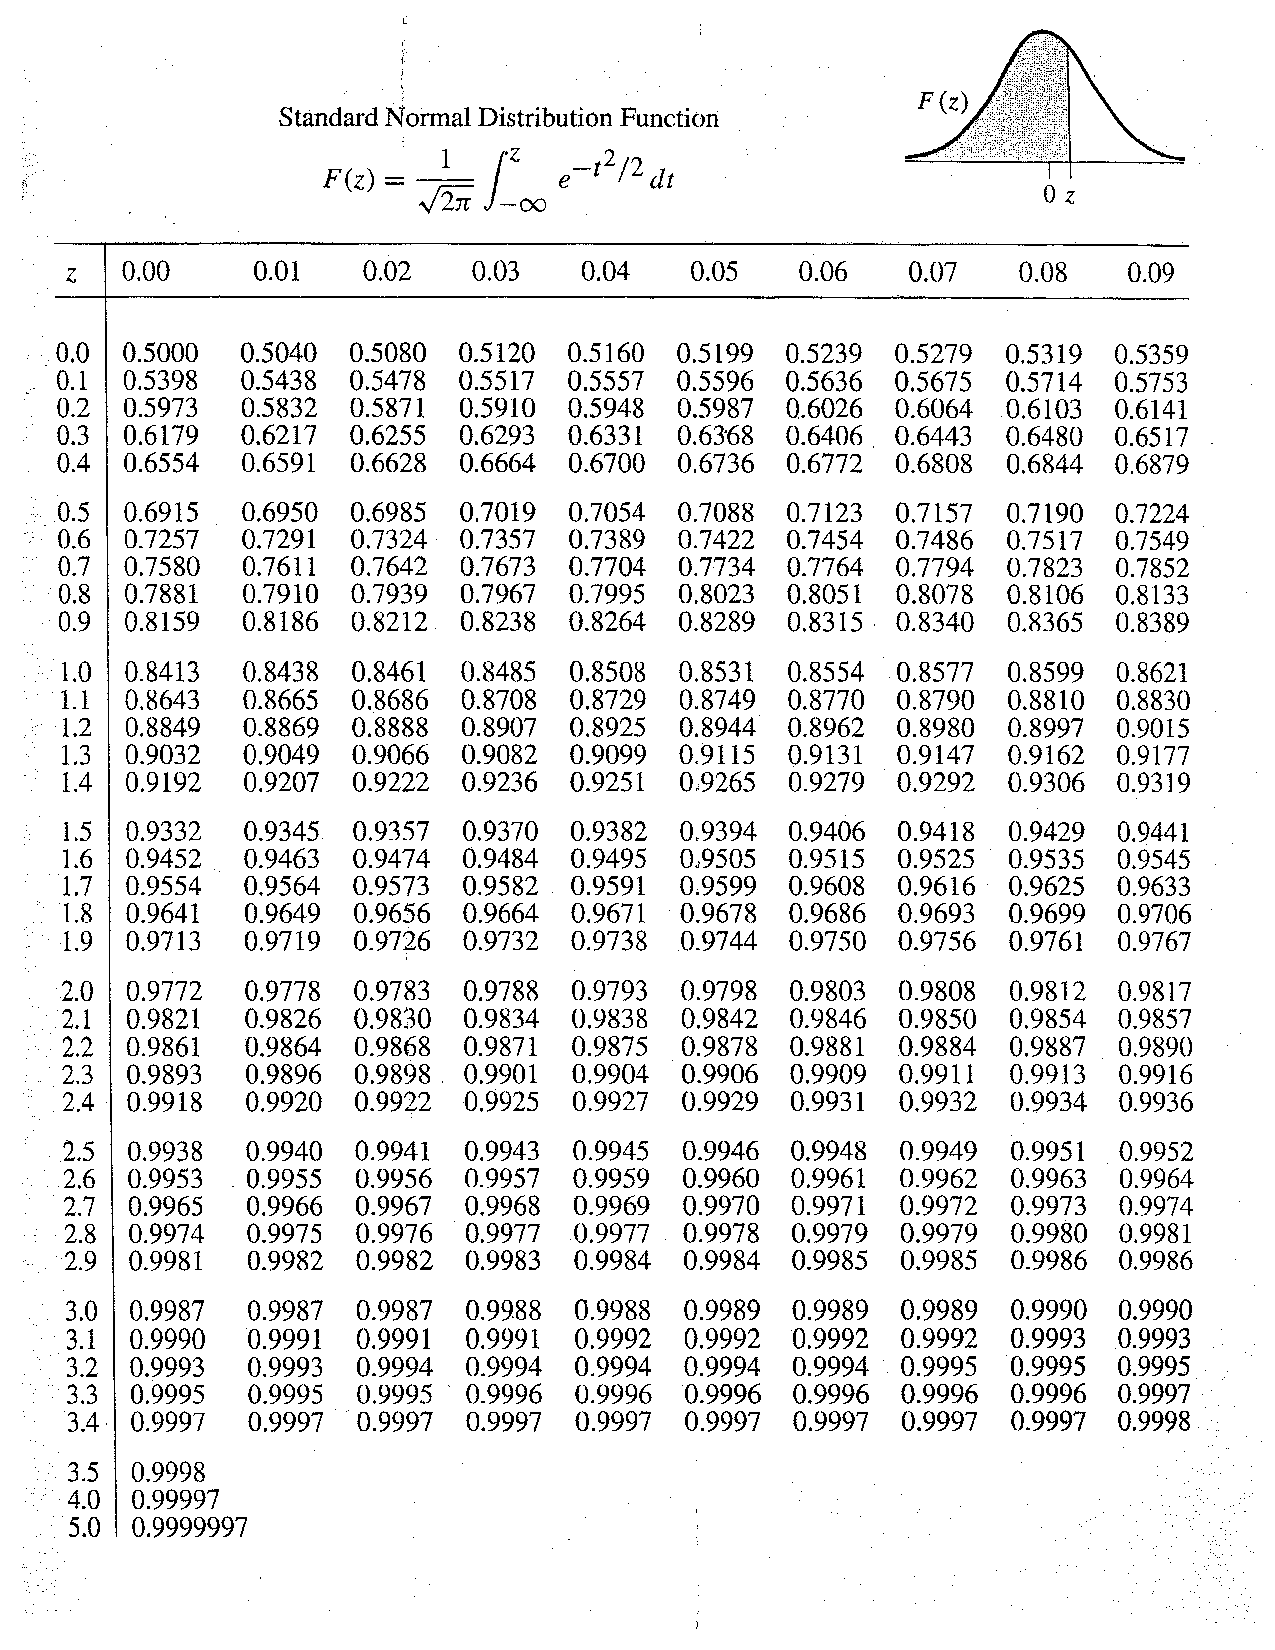
\includegraphics[
                % page=1,
                width=\textwidth,
                height=\textheight*2/3,
                keepaspectratio
            ]{tables/standard_normal_probability_table.pdf}
            \vfill
        \newpage
    % chapter normal_distribution_table (end)
    \chapter{Chi-Squared Table} % (fold)
    \label{cha:chi_squared_table}
        % \newpage
        \noindent
            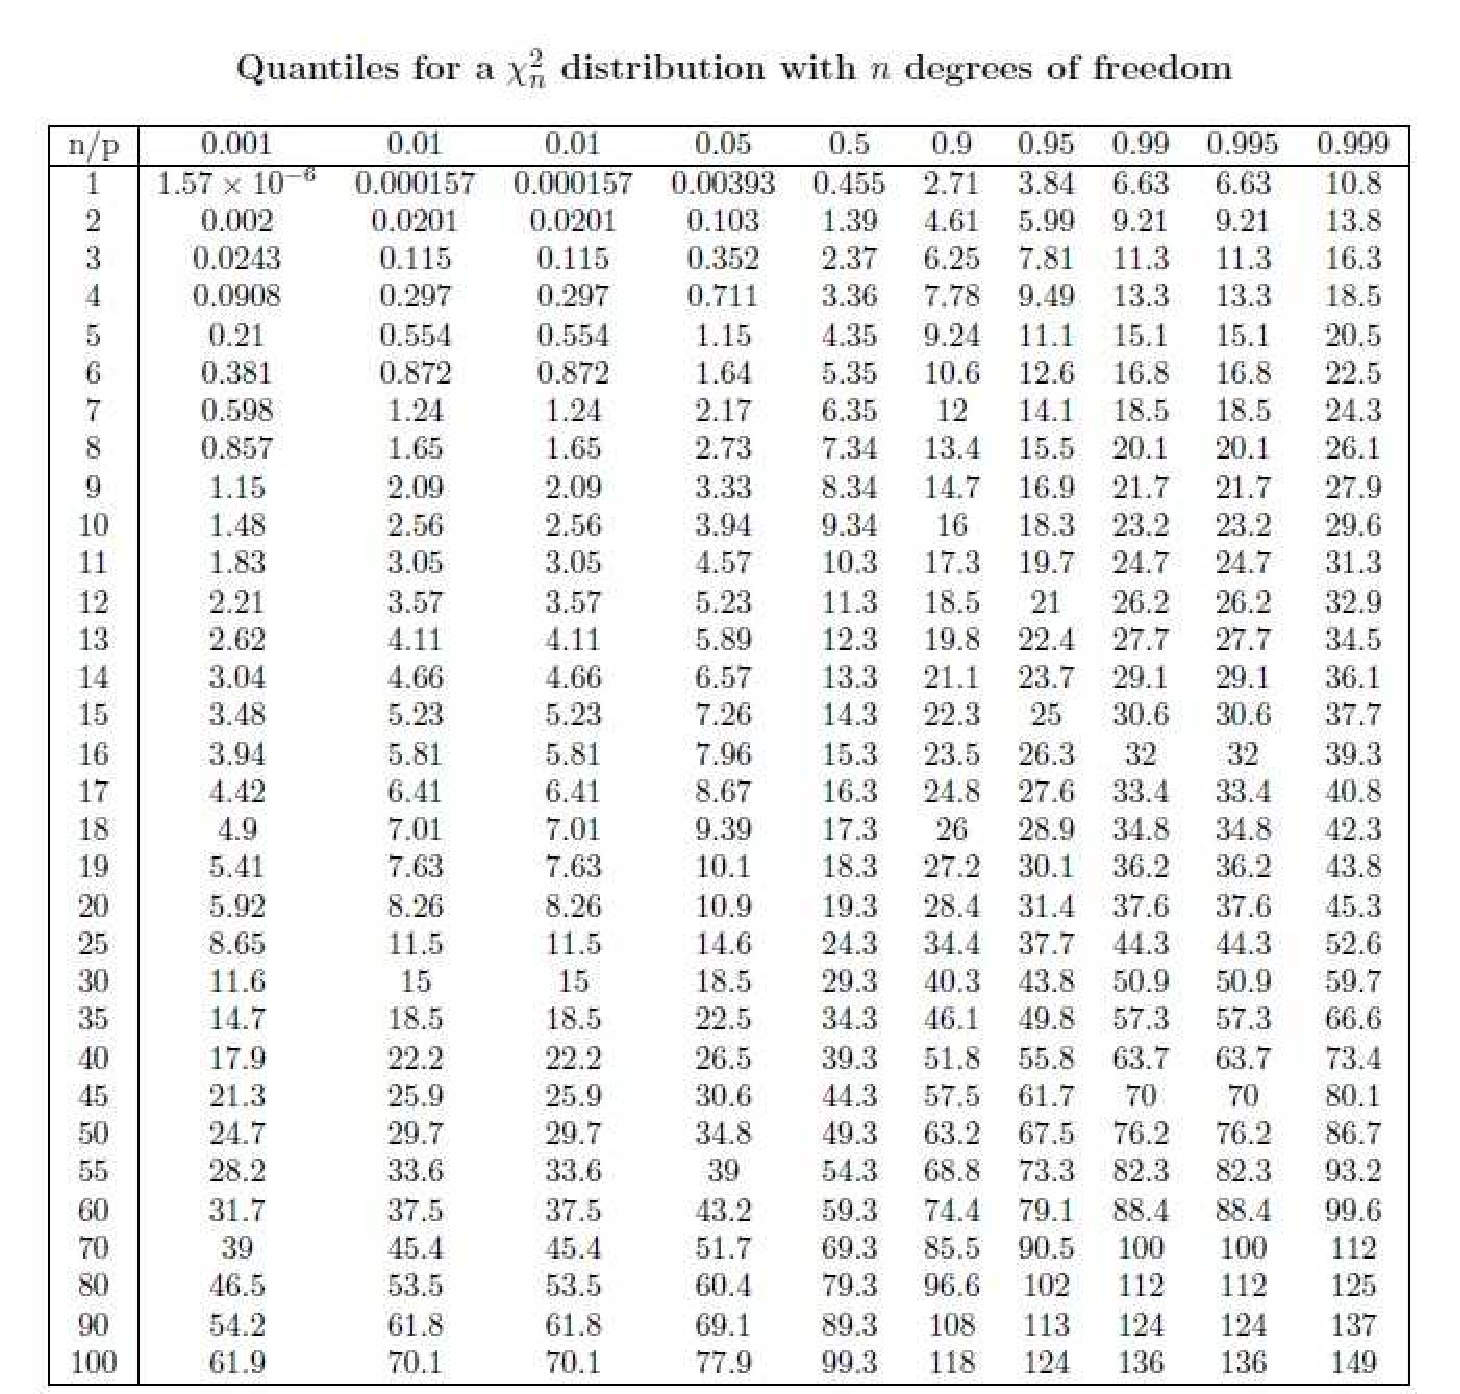
\includegraphics[
                % page=1,
                width=\textwidth,
                height=\textheight*2/3,
                keepaspectratio
            ]{tables/chi_squared_table.pdf}
            \vfill
        \newpage
    % chapter chi_squared_table (end)
    \chapter{Student-T Reference Table} % (fold)
    \label{cha:student_t_reference_table}
        % \newpage
        \noindent
            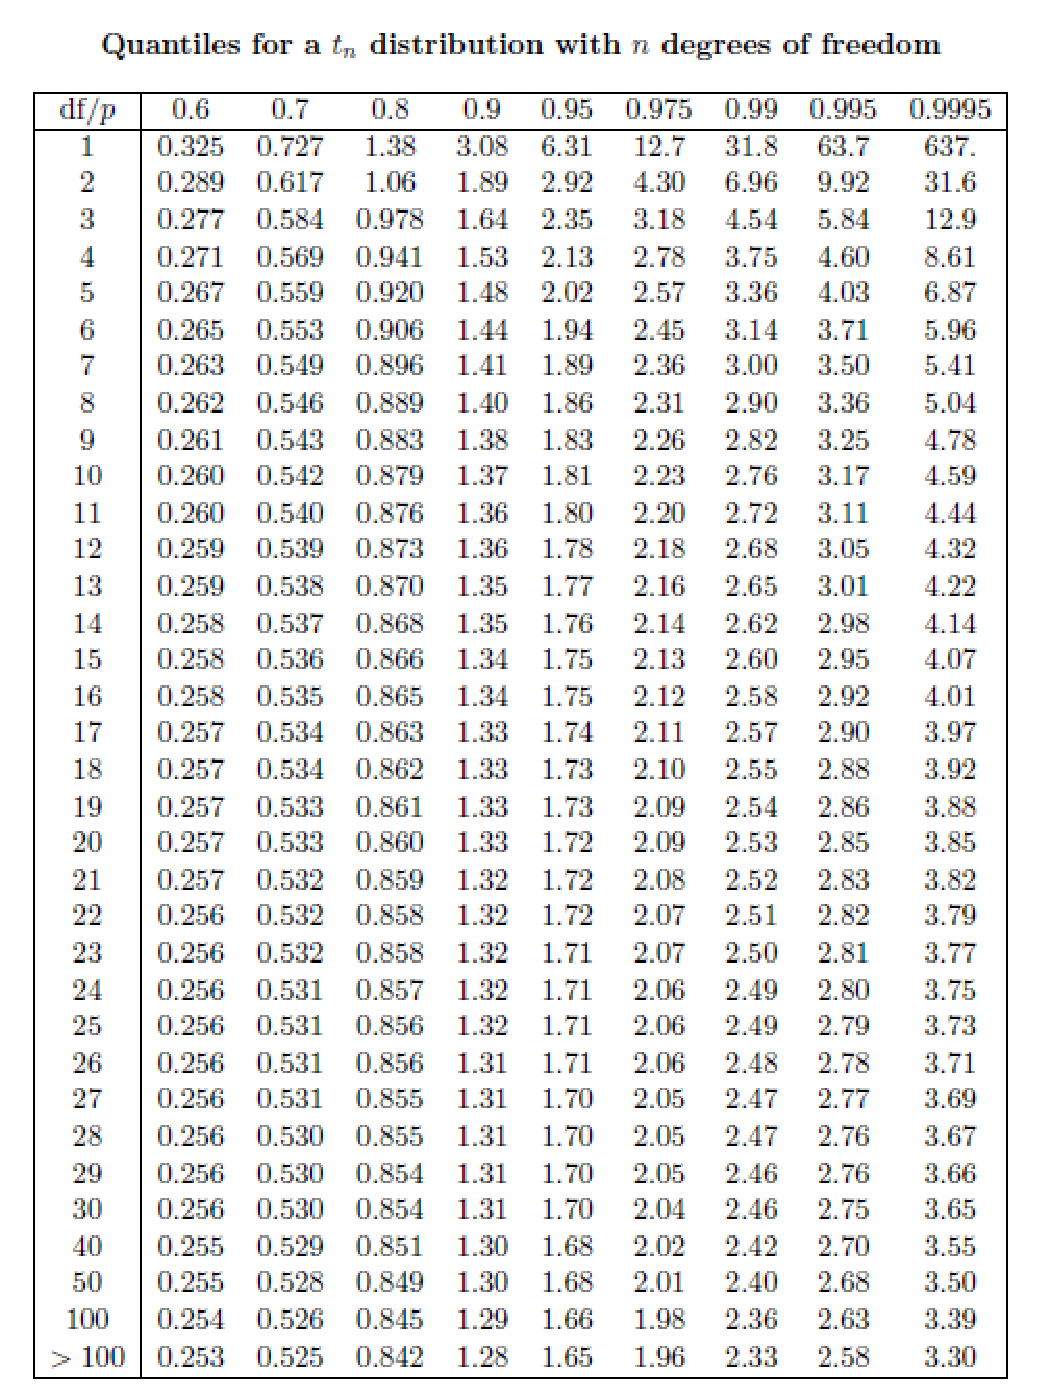
\includegraphics[
                % page=1,
                width=\textwidth,
                height=\textheight*2/3,
                keepaspectratio
            ]{tables/student_t_reference_table.pdf}
            \vfill
        \newpage
    % chapter student_t_reference_table (end)

\newpage

\printindex

\end{document}

